\documentclass[11pt,oneside]{article}
\usepackage[T1]{fontenc}
\usepackage[utf8]{inputenc}
% \usepackage{lmodern}
%\usepackage[adobe-utopia,uppercase=upright,greeklowercase=upright]{mathdesign}
\usepackage[adobe-utopia]{mathdesign}
%\usepackage{minionpro}
% \usepackage{pifont}
% \usepackage{amssymb}
\usepackage{amsmath}
\usepackage[francais]{babel}
% \usepackage[francais]{varioref}
\usepackage[dvips]{graphicx}

\usepackage{framed}
\usepackage[normalem]{ulem}
\usepackage{fancyhdr}
\usepackage{titlesec}
\usepackage{vmargin}
\usepackage{longtable}

\usepackage{ifthen}


%\usepackage{epsfig}
\usepackage{subfig}

\usepackage{multirow}
\usepackage{multicol} % Portions de texte en colonnes
\usepackage{flafter}%floatants après la référence



\usepackage{color}
\usepackage{colortbl}


\definecolor{gris25}{gray}{0.75}
\definecolor{bleu}{RGB}{18,33,98}
\definecolor{bleuf}{RGB}{42,94,171}
\definecolor{bleuc}{RGB}{231,239,247}
\definecolor{rougef}{RGB}{185,18,27}
\definecolor{rougec}{RGB}{255,230,231}
\definecolor{vertf}{RGB}{103,126,82}
\definecolor{vertc}{RGB}{220,255,191}

\newenvironment{rem}[1][\hsize]%
{%
    \def\FrameCommand
    {%
\rotatebox{90}{\textit{\textsf{Remarque}}} 
        {\color{bleuf}\vrule width 3pt}%
        \hspace{0pt}%must no space.
        \fboxsep=\FrameSep\colorbox{bleuc}%
    }%
    \MakeFramed{\hsize#1\advance\hsize-\width\FrameRestore}%
}%
{\endMakeFramed}%


\newenvironment{savoir}[1][\hsize]%
{%
    \def\FrameCommand
    {%
\rotatebox{90}{\textit{\textsf{Savoir}}} 
        {\color{bleuf}\vrule width 3pt}%
        \hspace{0pt}%must no space.
        \fboxsep=\FrameSep\colorbox{bleuc}%
    }%
    \MakeFramed{\hsize#1\advance\hsize-\width\FrameRestore}%
}%
{\endMakeFramed}%

\newenvironment{prob}[1][\hsize]%
{%
    \def\FrameCommand%
    {%
\rotatebox{90}{\textit{\textsf{ Problématique}}} 
        {\color{rougef}\vrule width 3pt}%
        \hspace{0pt}%must no space.
        \fboxsep=\FrameSep\colorbox{rougec}%
    }%
    \MakeFramed{\hsize#1\advance\hsize-\width\FrameRestore}%
}%
{\endMakeFramed}%

\newenvironment{obj}[1][\hsize]%
{%
    \def\FrameCommand%
    {%
\rotatebox{90}{\textit{\textsf{ $\;$}}} 
        {\color{rougef}\vrule width 3pt}%
        \hspace{0pt}%must no space.
        \fboxsep=\FrameSep\colorbox{rougec}%
    }%
    \MakeFramed{\hsize#1\advance\hsize-\width\FrameRestore}%
}%
{\endMakeFramed}%

\newenvironment{defi}[1][\hsize]%
{%
    \def\FrameCommand%
    {%
\rotatebox{90}{\textit{\textsf{Définition\\}}} 
        {\color{bleuf}\vrule width 3pt}%
        \hspace{0pt}%must no space.
        \fboxsep=\FrameSep\colorbox{bleuc}%
    }%
    \MakeFramed{\hsize#1\advance\hsize-\width\FrameRestore}%
}%
{\endMakeFramed}%


\newenvironment{hypo}[1][\hsize]%
{%
    \def\FrameCommand%
    {%
\rotatebox{90}{\textit{\textsf{Hypothèse\\}}} 
        {\color{bleuf}\vrule width 3pt}%
        \hspace{0pt}%must no space.
        \fboxsep=\FrameSep\colorbox{bleuc}%
    }%
    \MakeFramed{\hsize#1\advance\hsize-\width\FrameRestore}%
}%
{\endMakeFramed}%


\newenvironment{prop}[1][\hsize]%
{%
    \def\FrameCommand%
    {%
\rotatebox{90}{\textit{\textsf{Propriété\\}}} 
        {\color{bleuf}\vrule width 3pt}%
        \hspace{0pt}%must no space.
        \fboxsep=\FrameSep\colorbox{bleuc}%
    }%
    \MakeFramed{\hsize#1\advance\hsize-\width\FrameRestore}%
}%
{\endMakeFramed}%

\newenvironment{props}[1][\hsize]%
{%
    \def\FrameCommand%
    {%
\rotatebox{90}{\textit{\textsf{Propriétés\\}}} 
        {\color{bleuf}\vrule width 3pt}%
        \hspace{0pt}%must no space.
        \fboxsep=\FrameSep\colorbox{bleuc}%
    }%
    \MakeFramed{\hsize#1\advance\hsize-\width\FrameRestore}%
}%
{\endMakeFramed}%

\newenvironment{exemple}[1][\hsize]%
{%
    \def\FrameCommand%
    {%
\rotatebox{90}{\textit{\textsf{Exemple\\}}} 
        {\color{vertf}\vrule width 3pt}%
        \hspace{0pt}%must no space.
        \fboxsep=\FrameSep\colorbox{vertc}%
    }%
    \MakeFramed{\hsize#1\advance\hsize-\width\FrameRestore}%
}%
{\endMakeFramed}%

\newenvironment{resultat}[1][\hsize]%
{%
    \def\FrameCommand%
    {%
\rotatebox{90}{\textit{\textsf{Résultat\\}}} 
        {\color{rougef}\vrule width 3pt}%
        \hspace{0pt}%must no space.
        \fboxsep=\FrameSep\colorbox{rougec}%
    }%
    \MakeFramed{\hsize#1\advance\hsize-\width\FrameRestore}%
}%
{\endMakeFramed}%

\newenvironment{methode}[1][\hsize]%
{%
    \def\FrameCommand%
    {%
\rotatebox{90}{\textit{\textsf{Méthode\\}}} 
        {\color{rougef}\vrule width 3pt}%
        \hspace{0pt}%must no space.
        \fboxsep=\FrameSep\colorbox{rougec}%
    }%
    \MakeFramed{\hsize#1\advance\hsize-\width\FrameRestore}%
}%
{\endMakeFramed}%

\newenvironment{theo}[1][\hsize]%
{%
    \def\FrameCommand%
    {%
\rotatebox{90}{\textit{\textsf{Théorème\\}}} 
        {\color{rougef}\vrule width 3pt}%
        \hspace{0pt}%must no space.
        \fboxsep=\FrameSep\colorbox{rougec}%
    }%
    \MakeFramed{\hsize#1\advance\hsize-\width\FrameRestore}%
}%
{\endMakeFramed}%

\newenvironment{warn}[1][\hsize]%
{%
    \def\FrameCommand%
    {%
\rotatebox{90}{\textit{\textsf{Attention\\}}} 
        {\color{rougef}\vrule width 3pt}%
        \hspace{0pt}%must no space.
        \fboxsep=\FrameSep\colorbox{rougec}%
    }%
    \MakeFramed{\hsize#1\advance\hsize-\width\FrameRestore}%
}%
{\endMakeFramed}%

% \usepackage{pstricks}
%\usepackage{minitoc}
% \setcounter{minitocdepth}{4}

\setcounter{tocdepth}{2}

% \mtcselectlanguage{french} 

%\usepackage{draftcopy}% "Brouillon"
% \usepackage{floatflt}
\usepackage{psfrag}
%\usepackage{listings} % Permet d'insérer du code de programmation
\renewcommand{\baselinestretch}{1.2}

% Changer la numérotation des figures :
% ------------------------------------
% \makeatletter
% \renewcommand{\thefigure}{\ifnum \c@section>\z@ \thesection.\fi
%  \@arabic\c@figure}
% \@addtoreset{figure}{section}
% \makeatother
 


%%%%%%%%%%%%
% Définition des vecteurs %
%%%%%%%%%%%%
 \newcommand{\vect}[1]{\overrightarrow{#1}}

%%%%%%%%%%%%
% Définition des torseusr %
%%%%%%%%%%%%

 \newcommand{\torseur}[1]{%
\left\{{#1}\right\}
}

\newcommand{\torseurcin}[3]{%
\left\{\mathcal{#1} \left(#2/#3 \right) \right\}
}

\newcommand{\torseurstat}[3]{%
\left\{\mathcal{#1} \left(#2\rightarrow #3 \right) \right\}
}

 \newcommand{\torseurc}[8]{%
%\left\{#1 \right\}=
\left\{
{#1}
\right\}
 = 
\left\{%
\begin{array}{cc}%
{#2} & {#5}\\%
{#3} & {#6}\\%
{#4} & {#7}\\%
\end{array}%
\right\}_{#8}%
}

 \newcommand{\torseurcol}[7]{
\left\{%
\begin{array}{cc}%
{#1} & {#4}\\%
{#2} & {#5}\\%
{#3} & {#6}\\%
\end{array}%
\right\}_{#7}%
}

 \newcommand{\torseurl}[3]{%
%\left\{\mathcal{#1}\right\}_{#2}=%
\left\{%
\begin{array}{l}%
{#1} \\%
{#2} %
\end{array}%
\right\}_{#3}%
}

 \newcommand{\vectv}[3]{%
\vect{V\left( {#1} \in {#2}/{#3}\right)}
}


\newcommand{\vectf}[2]{%
\vect{R\left( {#1} \rightarrow {#2}\right)}
}

\newcommand{\vectm}[3]{%
\vect{\mathcal{M}\left( {#1}, {#2} \rightarrow {#3}\right)}
}


 \newcommand{\vectg}[3]{%
\vect{\Gamma \left( {#1} \in {#2}/{#3}\right)}
}

 \newcommand{\vecto}[2]{%
\vect{\Omega\left( {#1}/{#2}\right)}
}
% }$$\left\{\mathcal{#1} \right\}_{#2} =%
% \left\{%
% \begin{array}{c}%
%  #3 \\%
%  #4 %
% \end{array}%
% \right\}_{#5}}

%  ------------------------------------------
% | Modification du formatage des sections : | 
%  ------------------------------------------

% Grands titres :
% ---------------

\newcommand{\titre}[1]{%
\begin{center}
      \bigskip
      \rule{\textwidth}{1pt}
      \par\vspace{0.1cm}
      
      \textbf{\large #1}
      \par\rule{\textwidth}{1pt}
    \end{center}
    \bigskip
  }

% Supprime le numéro du chapitre dans la numérotation des sections:
% -----------------------------------------------------------------
\makeatletter
\renewcommand{\thesection}{\@arabic\c@section}
\makeatother


% \titleformat{\chapter}[display]
% {\normalfont\Large\filcenter}
% {}
% {1pc}
% {\titlerule[1pt]
%   \vspace{1pc}%
%   \Huge}[\vspace{1ex}%
% \titlerule]


%%%% Chapitres Comme PY Pechard %%%%%%%%%
% numéro du chapitre
\DeclareFixedFont{\chapnumfont}{OT1}{phv}{b}{n}{80pt}
% pour le mot « Chapitre »
\DeclareFixedFont{\chapchapfont}{OT1}{phv}{m}{it}{40pt}
% pour le titre
\DeclareFixedFont{\chaptitfont}{T1}{phv}{b}{n}{25pt}

\definecolor{gris}{gray}{0.75}
\titleformat{\chapter}[display]%
	{\sffamily}%
	{\filleft\chapchapfont\color{gris}\chaptertitlename\
	\\
	\vspace{12pt}
	\chapnumfont\thechapter}%
	{16pt}%
	{\filleft\chaptitfont}%
	[\vspace{6pt}\titlerule\titlerule\titlerule]

%%%%  Fin Chapitres Comme PY Pechard %%%%%%%%%


% Section, subsection, subsubsection sans serifs :
% % ----------------------------------------------

% \makeatletter
% \renewcommand{\section}{\@startsection{section}{0}{0mm}%
% {\baselineskip}{.3\baselineskip}%
% {\normalfont\sffamily\Large\textbf}}%
% \makeatother

\makeatletter
\renewcommand{\@seccntformat}[1]{{\textcolor{bleu}{\csname
the#1\endcsname}\hspace{0.5em}}}
\makeatother

\makeatletter
\renewcommand{\section}{\@startsection{section}{1}{\z@}%
                       {-4ex \@plus -1ex \@minus -.4ex}%
                       {1ex \@plus.2ex }%
                       {\normalfont\Large\sffamily\bfseries}}%
\makeatother
 
\makeatletter
\renewcommand{\subsection}{\@startsection {subsection}{2}{\z@}
                          {-3ex \@plus -0.1ex \@minus -.4ex}%
                          {0.5ex \@plus.2ex }%
                          {\normalfont\large\sffamily\bfseries}}
\makeatother
 
\makeatletter
\renewcommand{\subsubsection}{\@startsection {subsubsection}{3}{\z@}
                          {-2ex \@plus -0.1ex \@minus -.2ex}%
                          {0.2ex \@plus.2ex }%
                          {\normalfont\large\sffamily\bfseries}}
\makeatother
 
\makeatletter             
\renewcommand{\paragraph}{\@startsection{paragraph}{4}{\z@}%
                                    {-2ex \@plus-.2ex \@minus .2ex}%
                                    {0.1ex}%               
{\normalfont\sffamily\bfseries}}
\makeatother
 
\makeatletter
\renewcommand{\subparagraph}{\@startsection{subparagraph}{5}{\z@}%
                                       {-2ex \@plus-.1ex \@minus .2ex}%
                                       {0.1ex}%
				    {\normalfont\normalsize\sffamily\bfseries}}
\makeatletter
% \makeatletter
% \renewcommand{\subsection}{\@startsection{subsection}{1}{2mm}%
% {\baselineskip}{.3\baselineskip}%
% {\normalfont\sffamily\large\textbf}}%
% \makeatother
% 
% \makeatletter
% \renewcommand{\subsubsection}{\@startsection{subsubsection}{2}{4mm}%
% {\baselineskip}{.15\baselineskip}%
% {\normalfont\sffamily\large\textbf}}%
% \makeatother
% 
% \makeatletter
% \renewcommand{\paragraph}{\@startsection{paragraph}{3}{6mm}%
% {\baselineskip}{.15\baselineskip}%
% {\normalfont\sffamily\large\textbf}}%
% \makeatother
 
\setcounter{secnumdepth}{4}


%  --------
% | Marges |
%  --------


% \setmarginsrb{2.5cm}{1.5cm}{2.5cm}{2cm}{1cm}{1cm}{1cm}{1cm}
\setmarginsrb{1.5cm}{1cm}{1cm}{1.5cm}{1cm}{1cm}{1cm}{1cm}

% Changer les marges localement :
% -----------------------------
\newenvironment{changemargin}[2]{\begin{list}{}{%
\setlength{\topsep}{0pt}%
\setlength{\leftmargin}{0pt}%
\setlength{\rightmargin}{0pt}%
\setlength{\listparindent}{\parindent}%
\setlength{\itemindent}{\parindent}%
\setlength{\parsep}{0pt plus 1pt}%
\addtolength{\leftmargin}{#1}%
\addtolength{\rightmargin}{#2}%
}\item }{\end{list}}



\usepackage{pst-solides3d}
\usepackage{titletoc}
\titlecontents{chapter}[+3pc]
  {\addvspace{10pt}\sffamily\bfseries}
{\contentslabel[{\pscirclebox[fillstyle=solid,fillcolor=gray!25,
linecolor=gray!25,framesep=4pt]{\textcolor{white}{\thecontentslabel}}}]{2.5pc}}
  {}
  {\dotfill \normalfont\thecontentspage\ }

\titlecontents{section}[3pc]
  {\addvspace{2pt}\sffamily}
  {\contentslabel[\thecontentslabel]{1.8pc}}
  {}
  {\dotfill \normalfont\thecontentspage\ }

\titlecontents{subsection}[5pc]
  {\addvspace{2pt}\sffamily}
  {\contentslabel[\thecontentslabel]{1.8pc}}
  {}
  {\dotfill \normalfont\thecontentspage\ }

\titlecontents{subsubsection}[8pc]
  {\addvspace{2pt}\sffamily}
  {\contentslabel[\thecontentslabel]{3pc}}
  {}
  {\dotfill \normalfont\thecontentspage\ }
%{\;\titlerule\;\normalfont\thecontentspage\ }

\titlecontents{paragraph}[9pc]
  {\addvspace{2pt}\sffamily}
  {\contentslabel[\thecontentslabel]{3.5pc}}
  {}
  {\dotfill \normalfont\thecontentspage\ }




\usepackage[%
    pdftitle={TD Statique},
    pdfauthor={Xavier Pessoles},
    colorlinks=true,
    linkcolor=blue,
    citecolor=magenta]{hyperref}



% \makeatletter \let\ps@plain\ps@empty \makeatother
%% DEBUT DU DOCUMENT
%% =================
\sloppy
\hyphenpenalty 10000

\newcommand{\Pointilles}[1][3]{%
\multido{}{#1}{\makebox[\linewidth]{\dotfill}\\[\parskip]
}}


\begin{document}


\newboolean{prof}
\setboolean{prof}{false}
%------------- En tetes et Pieds de Pages ------------
\pagestyle{fancy}
\renewcommand{\headrulewidth}{0pt}

\fancyhead{}
\fancyhead[L]{%
\begin{minipage}[c]{1.6cm}

\includegraphics[width=1.4cm]{png/logo_jh_ptsi.png}%
\end{minipage}
\rule{2cm}{.5pt}
}

\fancyhead[C]{\rule{12cm}{.5pt}}

\fancyhead[R]{%
\begin{minipage}[c]{3cm}
\begin{flushright}
\footnotesize{\textit{\textsf{Sciences Industrielles\\ pour l'Ingénieur}}}%
\end{flushright}
\end{minipage}
}

\renewcommand{\footrulewidth}{0.2pt}

\fancyfoot[C]{\footnotesize{\bfseries \thepage}}
\fancyfoot[L]{\footnotesize{2011 -- 2012} \\ X. \textsc{Pessoles}}
\ifthenelse{\boolean{prof}}{%
\fancyfoot[R]{\footnotesize{TD -- CI 3 : Statique -- P}}
}{%
\fancyfoot[R]{\footnotesize{TD -- CI 3 : Statique}}
}


%\begin{center}
%\textit{Centre d'intérêt}
%\end{center}

\begin{center}
 \huge\textsc{CI 3 -- Statique : Modélisation, prévision et vérification du comportement statique des systèmes}
\end{center}

\begin{center}
 \LARGE\textsc{Chapitre 3 -- Étude graphique} 
\end{center}

%\setcounter{paragraph}{0}
\vspace{.5cm}

\section*{Porte d'autobus}

On considère un système d'ouverture de porte d'autobus dont on donne un extrait du cahier des charges ci-dessous.

\begin{center}
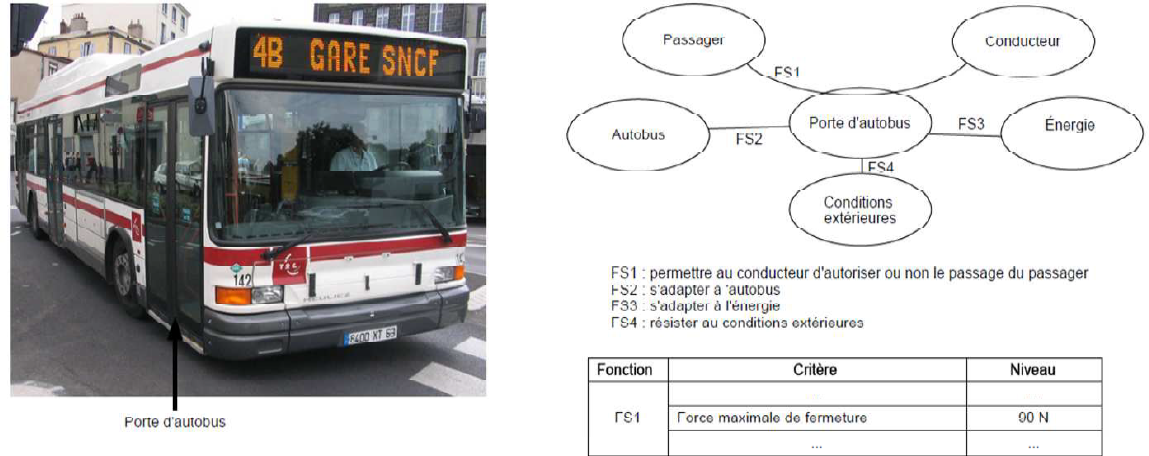
\includegraphics[width=.9\textwidth]{png/img1.png}
\end{center}

(L'effort maximal de fermeture est de 90\; N).

La figure de la page suivante représente le schéma du mécanisme actionneur d'une porte (3) d'autobus (en vue de dessus). Au dessus de la porte, un vérin pneumatique (air comprimé) (4,5) entraîne une bielle (2) en liaison pivot avec la carrosserie (1). Le bras (AB), encastré à la bielle (2), entraîne une le battant de porte (3) qui est guide par une maneton (C) se déplaçant dans une rainure. L'amplitude de rotation de la bielle (2) de 90 degrés environ permet d'obtenir les positions extrêmes (ouvert/fermé) du battant (3). Tous les tracés se feront sur le document réponse de la page suivante. 

Lorsque la porte se ferme, il ne faut pas qu'elle exerce une force trop importante si jamais un passager venait à se faire coincer par elle. L'objectif est donc de vérifier si la porte d'autobus satisfait le niveau du critère de force maximale de fermeture de la fonction FS1 ou non.

Tous les tracés graphiques se feront sur la figure de la page suivante. 

\paragraph{}
\textit{En isolant la pièce 3, déterminer graphiquement les efforts dans les liaisons en $B$ et $C$. Faire les constructions graphiques en rouge.}

\paragraph{}
\textit{Déterminer la direction de l'effort dans la liaison $F$ en argumentant.}

\paragraph{}
\textit{En isolant la pièce 2, déterminer graphiquement les efforts dans les liaisons en $A$ et $F$. Faire les constructions graphiques en bleu.}

\paragraph{}
\textit{Déterminer si haute pression est dans la cavité intérieure gauche ou droite du vérin.}

\paragraph{}
\textit{La surface du piston $S=3cm^2$, et la pression dans le vérin étant limité à 1 MPa, conclure quant à la capacité de la porte d'autobus à satisfaire le niveau du critère de force maximale de fermeture de la fonction FS1.}

\newpage

 $\;$

\vspace{15cm}

\begin{center}
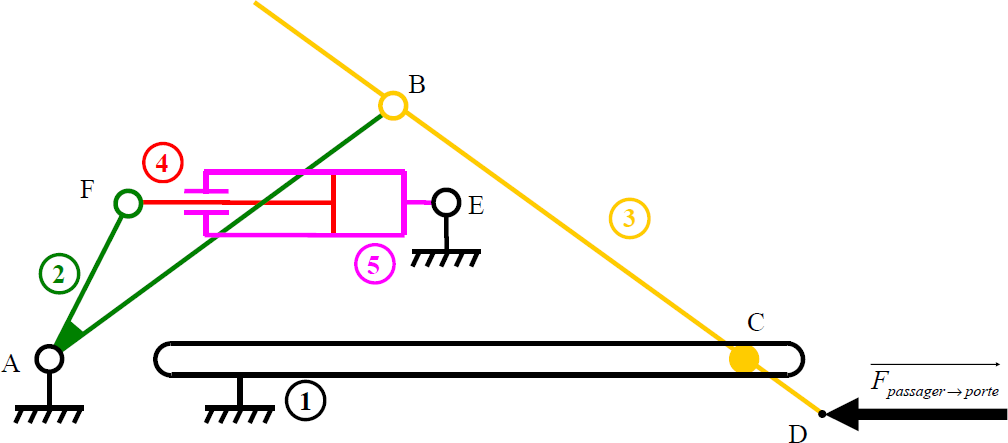
\includegraphics[width=.9\textwidth]{png/img2.png}
\end{center}

\newpage

\section*{Barrage de la Tamise}
\setcounter{paragraph}{0}

Le Thames Barrier est un barrage spectaculaire conçu pour protéger la ville de Londres des marées exceptionnellement élevées qui peuvent remonter de la mer. Sa construction terminée en 1982 a nécessité $51\;000$ tonnes d'acier $210\;000 \; m^3$ de béton, ce qui en fait le deuxième barrage mobile le plus grand du monde. 

\begin{center}
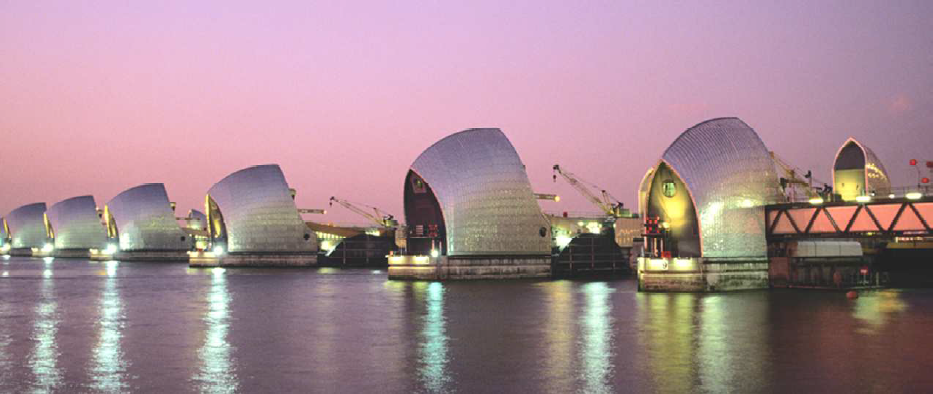
\includegraphics[width=.4\textwidth]{png/img3.png}
\end{center}

La structure s'étend sur 520 mètres de large et est constituée de 10 portes en forme de secteur angulaire de 20 mètres de haut. Chaque porte est totalement effacée dans un berceau en béton coulé au fond de la rivière. En cas de montée des eaux, les portes pivotent en position verticale par une machinerie hydraulique. 

\begin{center}
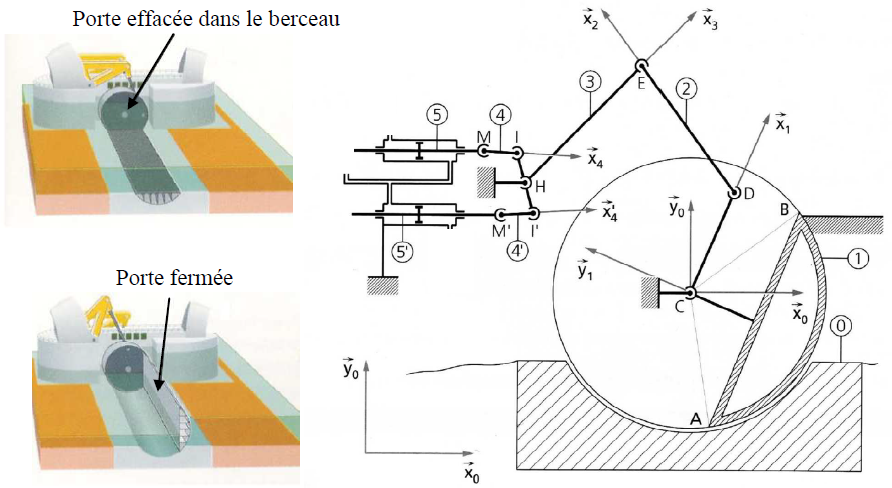
\includegraphics[width=.9\textwidth]{png/img4.png}
\end{center}

\begin{center}
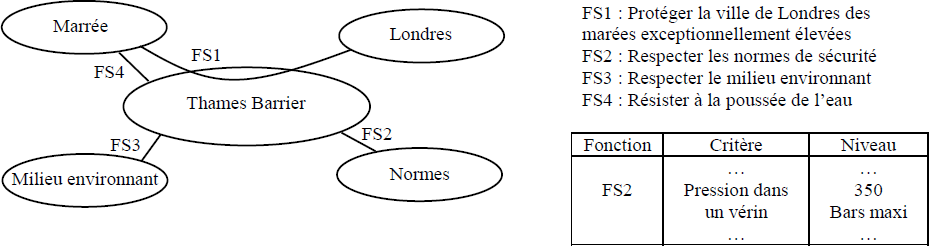
\includegraphics[width=.9\textwidth]{png/img5.png}
\end{center}

Le système qui peut être considéré comme plan est constitué de : 
\begin{itemize}
\item la porte 1 en liaison pivot d'axe $(C,\vect{z_0})$ avec le bâti 0 actionnée par la biellette 2 au niveau du point $D$;
\item la biellette 2 en liaison pivot d'axe $(D,\vect{z_0})$ avec la porte 1 et en liaison pivot d'axe $(E,\vect{z_0})$ avec la pièce 3;
\item la pièce 3 en liaison pivot d'axe $(H,\vect{z_0})$ avec le bâti 0 actionnée en I et I' par les biellettes 4 et 4';
\item les biellettes 4 et 4' en liaison pivot d'axe $(I,\vect{z_0})$ et d'axe $(I',\vect{z_0})$ avec les pièces 2 et en liaison pivot d'axe $(M,\vect{z_0})$ et $(M',\vect{z_0})$ avec les tiges des vérins 5 et 5';
\item deux vérins dont les tiges 5 et 5' actionnent les biellettes 4 et 4'. 
\end{itemize}

L'objectif et de vérifier ou non le critère de la FS2 dans le cas extrême où \textbf{seule la tige du vérin 5 est active suite à une rupture de la biellette 4'}.

\paragraph{} 
\textit{L'action mécanique de l'eau sur la porte est modélisée globalement par une force $\vect{F_{eau\rightarrow 1}}$ telle que : $\vect{F_{eau\rightarrow 1}}=\left[\begin{array}{c}
-2\cdot10^{6}\; N \\
-1\cdot10^{6}\; N \\ 
0\; N 
\end{array}\right]_{(\vect{x_0},\vect{y_0},\vect{z_0})}$. Déterminer dans la position représentée graphiquement l'action mécanique de la biellette 4 sur la tige de vérin 5.}

\paragraph{} 
\textit{Pour un diamètre de piston de 300\; mm, déterminer la pression dans la chambre de vérin et conclure vis-à-vis du Cahier des Charges Fonctionnel.}


\begin{center}
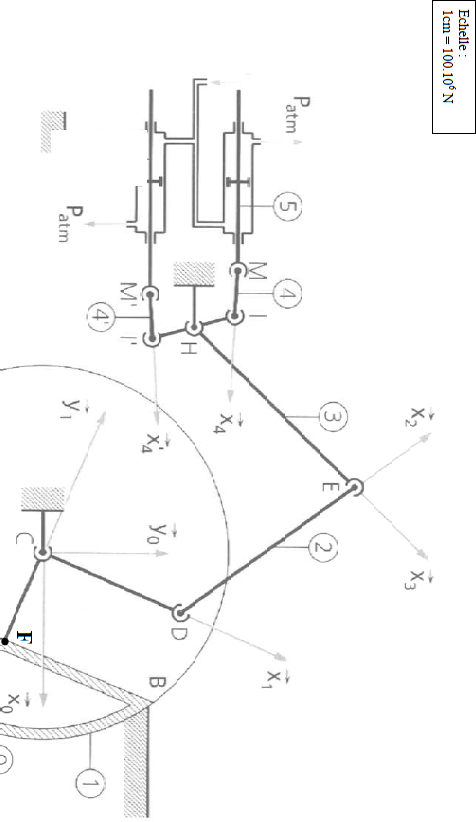
\includegraphics[height=.9\textheight]{png/img6.png}
\end{center}

\section*{Cric hydraulique}
\setcounter{paragraph}{0}
Un cric hydraulique étudié est utilise pour soulever une voiture afin de réaliser des opérations de maintenance. Le système est actionné par un vérin hydraulique piloté par une pompe hydraulique à commande manuelle. L'objectif est de vérifier le critère de force maximale à déployer de la fonction FS1. 


\begin{center}
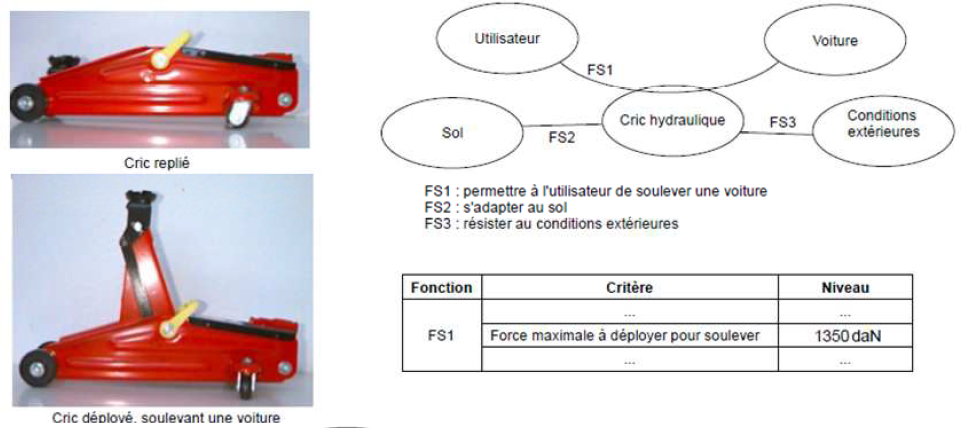
\includegraphics[width=.9\textwidth]{png/img7.png}
\end{center}


\begin{center}
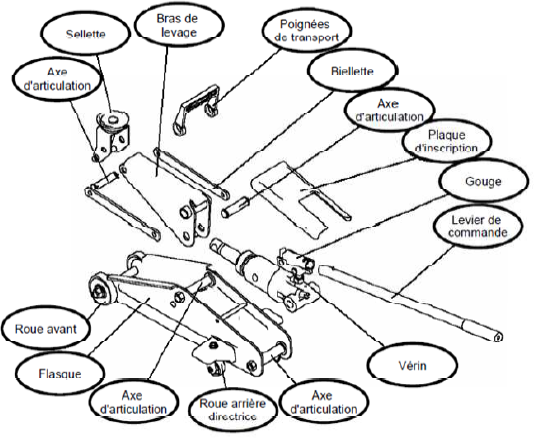
\includegraphics[width=.9\textwidth]{png/img8.png}
\end{center}

Le cric repose sur le sol. La voiture est en appui sur une sellette. L'utilisateur appuie sur un vérin de commande ce qui met en pression l'huile d'un vérin et crée les efforts nécessaires pour soulever la voiture. Un mécanisme de transformation du mouvement \{bras de levage+biellette\} permet d'adapter l'effort. Le vérin 4 est constitué de de deux pièces : le corps du vérin et la tige du vérin. La liaison entre ces deux pièces peut être modélisée par une liaison pivot glissant (ou glissière dans le plan). D'autre part, l'huile présente dans le vérin exerce une force sur ces deux pièces. La voiture exerce la force $P$ sur la sellette 3, et on recherche la pression de l'huile dans le vérin. 

Tous les tracés graphiques se feront sur le document suivant.

Description des liaisons : 
\begin{itemize}
\item bras de levage 2 et sellette 3 : pivot en $G$;
\item bras de levage 2 et bâti 1 : pivot en $E$;
\item bras de levage 2 et vérin 4 : pivot en $D$;
\item bâti 1 et biellette 5 : pivot en $H$;
\item sellette 3 et biellette 5 : pivot en $F$;
\item vérin 4 et bâti 1 : pivot en $C$.
\end{itemize}

\paragraph{}
\textit{Tracer le graphe d'analyse du système. Faire apparaître la force $P$.}

\paragraph{}
\textit{Ajouter sur le document réponse les numéros de pièces correspondant ainsi que les points des différentes liaisons.}

\paragraph{}
\textit{Déterminer la direction des actions mécaniques s'exerçant sur 5.}

\paragraph{}
\textit{Déterminer l'ensemble des actions mécaniques exercées sur 3. Réaliser les tracés en rouge sur le document réponse.}

\paragraph{}
\textit{Déterminer la direction des actions mécaniques s'exerçant sur 4.}

\paragraph{}
\textit{Déterminer l'ensemble des actions mécaniques s'exerçant sur 2. Réaliser les tracés en bleu sur le document réponse. }

\paragraph{}
\textit{Déterminer la norme de la force exercée par l'huile sur la tige du vérin, de section $28 cm^2$, lorsque $P$ a la valeur de la force maximale pour soulever de la fonction FS1.}

\paragraph{}
\textit{L'utilisateur, par son action sur le levier de commande, met l'huile sous pression, jusqu'à une valeur de 200 bars. Conclure quant à la capacité du cric à satisfaire le critère de force maximale à déployer de la fonction FS1.}



\begin{center}
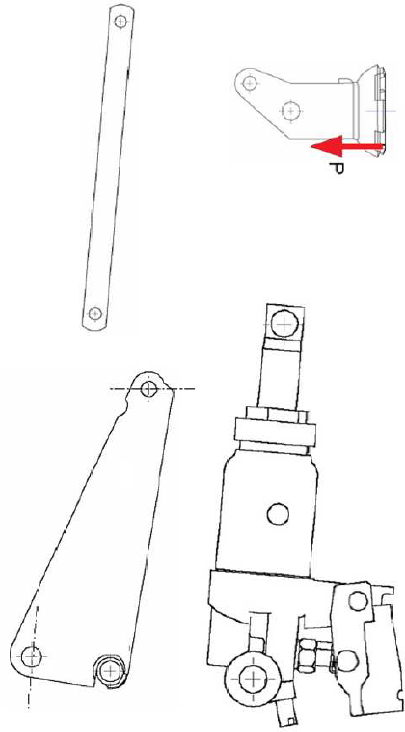
\includegraphics[height=.9\textheight]{png/img9.png}
\end{center}




\end{document}